% ------------------------------------------------------------------------
% ------------------------------------------------------------------------
% ICMC: Modelo de Trabalho Acadêmico (tese de doutorado, dissertação de
% mestrado e trabalhos monográficos em geral) em conformidade com 
% ABNT NBR 14724:2011: Informação e documentação - Trabalhos acadêmicos -
% Apresentação
% ------------------------------------------------------------------------
% ------------------------------------------------------------------------

% Opções: 
%   Qualificação          = qualificacao 
%   Curso                 = doutorado/mestrado
%   Situação do trabalho  = pre-defesa/pos-defesa (exceto para qualificação)
%   Versão para impressão = impressao
\documentclass[mestrado, pós-defesa]{packages/icmc}

% ---------------------------------------------------------------------------
% Pacotes Opcionais
% ---------------------------------------------------------------------------
\usepackage{rotating}           % Usado para rotacionar o texto
\usepackage[all,knot,arc,import,poly]{xy}   % Pacote para desenhos gráficos
% Este pacote pode conflitar com outros pacotes gráficos como o ``pictex''
% Então é necessário usar apenas um dos pacotes conflitantes
\newcommand{\VerbL}{0.52\textwidth}
\newcommand{\LatL}{0.42\textwidth}
% ---------------------------------------------------------------------------

\usepackage{placeins}
\usepackage{tabularx}
\usepackage{listings}
\usepackage{xcolor}

\definecolor{codegreen}{rgb}{0,0.6,0}
\definecolor{codegray}{rgb}{0.5,0.5,0.5}
\definecolor{codepurple}{rgb}{0.58,0,0.82}
\definecolor{backcolour}{rgb}{0.97,0.97,0.97}
\lstdefinestyle{mystyle}{
  backgroundcolor=\color{backcolour},   
  commentstyle=\color{codegreen},
  keywordstyle=\color{magenta},
  numberstyle=\minuscule\color{codegray},
  stringstyle=\color{codepurple},
  basicstyle=\ttfamily\tiny,
  breakatwhitespace=false,         
  breaklines=true,                 
  captionpos=b,                    
  keepspaces=true,                 
  numbers=left,                    
  numbersep=5pt,                  
  showspaces=false,                
  showstringspaces=false,
  showtabs=false,                  
  tabsize=2
}
\lstset{style=mystyle}

% ---
% Informações de dados para CAPA e FOLHA DE ROSTO
% ---
% Tanto na capa quanto nas folhas de rosto apenas a primeira letra da primeira palavra (ou nomes próprios) devem estar em letra maiúscula, todas as demais devem ser em letra minúscula.
\tituloPT{Um modelo de classificação para habilitar denúncias: um estudo de caso na CGU}
% \tituloEN{TODO: Modelo de Classificação de Risco de Denúncias}
\autor{Fernando Sola Pereira}
\genero{M} % Gênero do autor (M = Masculino / F = Feminino)
\orientador[Orientador]{Prof. Dr.}{Jó Ueyama}
%\coorientador{Prof. Dr.}{Fulano de Tal}
\curso{CCMC}
\data{17}{01}{2021} % Data do depósito
\idioma{PT} % Idioma principal do documento (PT = português / EN = inglês)
% ---


% ---
% RESUMOS
% ---

% Resumo em PORTUGUÊS
% conter no máximo 500 palavras
% conter no mínimo 1 e no máximo 5 palavras-chave
\textoresumo[brazil]{
Centenas de denúncias são enviadas diariamente através da Plataforma Integrada de Ouvidoria e Acesso à Informação (Fala.BR). Para que possam ser apuradas, primeiramente elas precisam ser triadas por uma equipe da Ouvidoria-Geral da União (OGU), área integrante da Controladoria-Geral da União (CGU), responsável por exercer as competências de órgão central do Sistema de Ouvidoria do Poder Executivo Federal. O processo de triagem consiste em avaliar se há o mínimo de informações necessárias presente na denúncia e, caso haja, encaminhar a denúncia para que uma área competente realize a apuração dos fatos denunciados.
Em média, apenas 30\% das denúncias que chegam são consideradas aptas pelos especialistas da Ouvidoria. Uma quantidade enorme de esforço é gasta pela equipe em denúncias que não possuem o mínimo de informação para qualquer tipo de apuração. O volume de denúncias é um obstáculo que exige uma grande equipe trabalhando no processo de triagem. Esta pesquisa propõe a criação de um modelo de classificação para habilitar denúncias, permitindo direcionar melhor os esforços das equipes responsáveis pelo processo de triagem.
}{Processamento de Linguagem Natural, Ciência de Dados}


% resumo em INGLÊS
% conter no máximo 500 palavras
% conter no mínimo 1 e no máximo 5 palavras-chave
% \textoresumo[english]{
%     TODO: This paper is a brief model for writing qualification monographs, dissertations and thesis using \LaTeX environment, in accordance with the standards required by the Institute of Mathematics and Computer Sciences (ICMC), University of São Paulo (USP). For making this model, the latest version (1.9.6) \textit{abnTeX2} classes package was used. This package follow the rules of the Brazilian Association of Technical Standards. A drafting a monograph, dissertation or thesis can be done by overwriting the contents of this model.
%     }{Template, Qualification monograph, Dissertation, Thesis, Latex}


% ----------------------------------------------------------
% ELEMENTOS PRÉ-TEXTUAIS
% ----------------------------------------------------------

% Inserir a ficha catalográfica
\incluifichacatalografica{tex/pre-textual/ficha-catalografica.pdf}

% DEDICATÓRIA / AGRADECIMENTO / EPÍGRAFE
% \textodedicatoria*{tex/pre-textual/dedicatoria}
% \textoagradecimentos*{tex/pre-textual/agradecimentos}
% \textoepigrafe*{tex/pre-textual/epigrafe}

% Inclui a lista de figuras
\incluilistadefiguras

% Inclui a lista de tabelas
\incluilistadetabelas

% Inclui a lista de quadros
% \incluilistadequadros

% Inclui a lista de algoritmos
% \incluilistadealgoritmos

% Inclui a lista de códigos
% \incluilistadecodigos

% Inclui a lista de siglas e abreviaturas
\incluilistadesiglas

% Inclui a lista de símbolos
% \incluilistadesimbolos

% ----
% Início do documento
% ----
\begin{document}
% ----------------------------------------------------------
% ELEMENTOS TEXTUAIS
% ----------------------------------------------------------
\textual

\chapter{Introdução}
\label{chapter:introducao}




No ambiente de negócios, o gerenciamento de reclamações de clientes tem se tornado um fator crítico de sucesso para manter um bom relacionamento e a fidelidade de clientes, conforme afirmam \citeonline{Coussement2008}. No ambiente da administração pública, onde o cidadão é o cliente, a prestação de serviços à população deve ser guiada por princípios como qualidade, eficiência e economicidade. Assim, diversos canais são disponibilizados aos cidadãos para entender melhor suas necessidades ou mesmo receber informações importantes sobre anomalias ou ilicitudes identificadas.

Centenas de denúncias são enviadas diariamente através da Plataforma Integrada de Ouvidoria e Acesso à Informação (Fala.BR). Para que possam ser apuradas, primeiramente elas precisam ser triadas por uma equipe da \sigla{OGU}{Ouvidoria-Geral da União}, área integrante da \sigla{CGU}{Controladoria-Geral da União}, responsável por exercer as competências de órgão central do Sistema de Ouvidoria do Poder Executivo federal. O processo de triagem consiste em avaliar se há o mínimo de informações necessárias presente na denúncia e, caso haja, encaminhar a denúncia para que uma área competente realize a apuração dos fatos denunciados.

Em média, apenas 30\% das denúncias que chegam são consideradas aptas pelos especialistas da Ouvidoria. Com isso, uma quantidade enorme de esforço é gasta pela equipe em denúncias que não possuem o mínimo de informação para qualquer tipo de apuração. O grande volume de denúncias é um obstáculo que exige uma grande equipe trabalhando no processo de triagem. 

Assim, a criação de um modelo de classificação que atribua o grau de risco de aptidão para uma denúncia permite direcionar melhor os esforços das equipes responsáveis pelo processo de triagem. O objetivo desta pesquisa é propor uma metodologia que permita a implementação deste modelo nos processo de triagem de  denúncias da OGU. 

O dados de denúncias recebidos através do sistema Fala.BR possuem poucos campos estruturados. A essência da denúncia está contida no texto escrito pelo cidadão e nos diversos anexos que, por vezes, são enviados em conjunto. Para uma pessoa, a análise de uma denúncia, na maioria das vezes é uma tarefa simples. Basicamente, o analista procura por elementos no texto que possam ser confirmados por consultas em sistemas oficiais como nomes de pessoas, números de cps, números de cnpj, endereços, órgãos, contratos, convênios, valores, além de outros elementos que possam remeter a uma certa gravidade sobre o problema exposto pelo cidadão. Entretanto, fazer este tipo de análise computacionalmente não é uma tarefa trivial. O \sigla{PLN}{Processamento de linguagem natural} é uma subárea da Ciência da Computação cujo o foco é a extração de informação. Este campo é vasto e é possível utilizar abordagens estatísticas como em \citeonline{Manning1999} ou combiná-las com abordagens simbólicas 


tial importance either because they suggest ways of combining statistical approaches with symbolic approaches (as in the regular-expression
post-filtering of collocations in (Justeson and Katz 1995b)) or because
the insights they offer can often be expressed in a statistical framework


Como abordarei o problema?

Para isso, será necessário compreender as diferentes formas de extrair informações de textos


Tema da Pesquisa ???
Delimitação do assunto ???

\chapter{Revisão Bibliográfica}
\label{chapter:revisao_bibliografica}

A utilização de reclamações e denúncias como subsídio para melhorar a qualidade dos serviços oferecidos pelo Estado é uma prática comum. Com a crescente evolução de técnicas e capacidade computacional nos últimos anos, é natural observar um aumento do seu emprego na automatização de processos relacionados à classificação e análise desse conjunto imenso de informações não estruturadas que chegam aos órgãos públicos constantemente. 

Na Alemanha explorou-se a ideia de que seria possível complementar modelos frequentemente utilizados em investigação forense eleitoral com informações de denúncias de cidadãos a respeito das eleições. Tais modelos utilizam métodos estatísticos, geralmente baseados em contagem de votos e na quantidade de eleitores elegíveis, para avaliar se os resultados de eleições refletem as intenções dos eleitores ou, ainda, avaliar se há indícios de fraudes no processo eleitoral. Conforme afirmam os autores do estudo, o uso dessas denúncias é uma forma de incorporar informação contextual e isso pode ser útil para avaliar e refinar os modelos existentes. Empregou-se diversas técnicas para tratar os textos das denúncias e por fim criou-se uma matriz de frequências de termos por documento. Com isso, foi possível criar um classificador que pudesse separar as denúncias de acordo com problema ou incidente endereçado por ela. A informação de classificação foi, então, utilizada para compor o modelo final proposto\cite{mebane2016frauds}.



\chapter{Modelo para classificar as denúncias}
\label{chapter:metodologia_proposta}
\section{Considerações Iniciais}

Neste capítulo pretende-se detalhar melhor o problema a ser resolvido. Posteriormente, será descrito todo o \textit{pipeline} de coleta e tratamentos dos dados para a montagem do conjunto de dados que será utilizado para treinamento e avaliação do modelo proposto.

\section{Detalhamento do Problema}

Ao chegar uma nova denúncia através do sistema FalaBR, da OGU, uma equipe de pessoas atua para avaliar as informações presentes na denúncia e decidir se a denúncia está apta a ser apurada ou não. Ou seja, a avaliação da equipe diz respeito a elementos presentes na denúncia que permitem uma apuração dos fatos relatados.

Em geral, estes elementos estão centrados em informações como CPF, CNPJ, Contratos e Convênios entre órgãos públicos e empresas privadas, materialidade (valores monetários descritos na denúncia ou identificados nos contratos e convênios). Com tais informações, a equipe de triagem de denúncias decide se deverá haver apuração (denúncia apta) ou não (denúncia não apta).

Uma grande parte deste trabalho pode ser automatizado. Assim, as consultas realizadas pela equipe, em diversos sistemas, podem ser substituídas por um processo automatizado, desde que seja possível identificar tais entidades no conteúdo das denúncias. Além disso, durante o processo de triagem, a equipe atribui uma nota de 0 a 100 (de 10 em 10) para definir o quão apta é uma denúncia. Por definições internas, notas entre 0 e 50 são consideradas não aptas e notas entre 60 e 100 são consideradas aptas. Tais notas podem ser utilizadas como rótulo para um aprendizado supervisionado.

Assim, sendo possível montar um conjunto de variáveis adequadas é possível propor a criação de um modelo para inferir notas às novas denúncias automaticamente.

O primeiro problema a ser resolvido, então, é a coleta e preparação dos dados. 
A próxima seção detalha os desafios enfrentados e como foram resolvidos.

\section{Coleta de Dados}

O processo de coleta e análise de dados para utilizar em treinamentos de aprendizado de máquina, geralmente, é composto por uma fase de análise exploratória. Em muitos casos, os dados estão estruturados e o maior trabalho é uma análise em que se verificam duplicidades, dados faltantes, \textit{outliers} e outras peculiaridades comuns em dados provenientes de sistemas informatizados. 
Já, no caso deste trabalho, não há, diretamente, dados estruturados. As únicas informações que podem ser obtidas são o texto da denúncia e os anexos, quando informados. Assim, a análise das denúncias e o seu uso para um aprendizado supervisionado devem abranger técnicas de NLP.

Como já foi mencionado, há rótulos sendo atribuídos às denúncias. Assim, o \textit{dataset} que será utilizado contém 1489 registros contendo informações da denúncia, anexos e a informação de grau de aptidão. Estes registros compreendem todas as denúncias cadastradas e que possuem rótulo atribuído entre 04/12/2019 e 23/06/2020.

\begin{figure}[htbp]
\caption{Quantidade de denúncias por rótulo}\label{fig_00100_quantidade_denuncias}
\begin{center}
    \includegraphics[width=\columnwidth]{images/fig_00100_quantidade_denuncias.png}
\end{center}
\legend{Fonte: Autor.}
\end{figure}

Conforme pode ser visto na \autoref{fig_00100_quantidade_denuncias}, a maior parte das denúncias recebeu um grau de aptidão 10, ou seja, são denúncias as quais os especialistas da OGU não possuem dúvidas de que as situações reportadas não devem ser apuradas.

\subsection{Extração de Textos dos Anexos}

Ao avaliar os anexos presentes em todas as denúncias cadastradas, identificou-se uma variedade muito grande de tipos de arquivos. Por essa razão, implementar um código, mesmo que utilizando bibliotecas prontas em Python \cite{rossum2009}, não se provou uma alternativa viável. Não foi possível identificar nenhuma biblioteca que conseguisse, sozinha, lidar com qualquer tipo de arquivo. Por outro lado, escrever um código para identificar o tipo de arquivo e realizar a chamada para uma biblioteca especializada no tipo de arquivo em questão não seria uma tarefa trivial e fugiria demais do escopo do trabalho.

Existe, no conjunto de dados avaliado por este trabalho, um total de 1801 anexos. A \autoref{fig_00050_quantidade_anexos_tipo_arquivo}, apresenta a quantidade de anexos de acordo com o tipo de arquivo.

\begin{figure}[htbp]
\caption{Quantidade de anexos por tipo de arquivo}
\label{fig_00050_quantidade_anexos_tipo_arquivo}
\begin{center}
\includegraphics[width=\columnwidth]{images/fig_00050_quantidade_anexos_tipo_arquivo.png}
\end{center}
\legend{Fonte: Autor.}
\end{figure}

Assim, para possibilitar a extração dos textos dos anexos, optou-se por utilizar uma ferramenta chamada Apache Tika (disponível em \url{http://tika.apache.org}) implementada em java. Esta ferramenta identifica automaticamente o tipo de arquivo e extrai o conteúdo textual e os metadados. A ferramenta, ainda, é capaz de realizar \sigla{OCR}{\textit{Optical Character Recognition}} quando há imagens dentro de arquivos dos tipo pdf, xls, doc, entre outros ou quando o arquivo é uma imagem.

Desta forma, configurou-se um servidor com a ferramenta instalada na forma de um serviço e utilizou-se uma biblioteca em Python para realizar as chamadas ao serviço passando os arquivos que deveriam ter o conteúdo extraído.

\subsection{Extração de Dados Estruturados}

A extração de dados estruturados é a tentativa de identificar certas entidades de interesse no conteúdo do texto da denúncia e seus anexos. As entidades de interesse, neste momento são CPF, CNPJ, convênios, contratos, NIS, nomes de pessoas, palavras fortes e valores.

Apesar de haver diversas formas de reconhecimento de entidades nomeadas, por questões de escopo e tempo, decidiu-se realizar a extração destas informações utilizando expressões regulares. A implementação de regras com expressões regulares para as entidades citadas acima, é simples na maioria dos casos e não exigem um treinamento como no caso dos algoritmos mencionados no \autoref{chapter:revisao_bibliografica}.

\subsection{Expansão das Informações}

Especialistas da OGU, ao analisar uma denúncia, pesquisam informações a partir do conteúdo das denúncias. Da mesma forma, a etapa de expansão compreende todos os dados estruturados, derivados daqueles encontrados na etapa anterior. 

Por exemplo, para um CPF citado, pode-se avaliar em quais CNPJs este CPF consta como sócio. Em um CNPJ pode-se avaliar os sócios. Em contratos ou convênios pode-se querer avaliar os participantes (órgãos e CNPJs), além do valor envolvido no ato administrativo. Para um nome de pessoa citado, pode-se tentar buscar o CPF caso não haja homônimos na base de CPFs da Receita Federal. Estas informações são extraídas e armazenadas mantendo-se a hierarquia, ou seja, um CNPJ extraído por que um CPF aparece no quadro societário possui um apontamento para o CPF que o originou e a relação ``é sócio de'' é preservada. Além disso, todos os dados estruturados preservam o identificador da denúncia a qual foram extraídos.

\begin{figure}[htbp]
    \caption{Exemplo de extração e expansão de dados estruturados}
    \label{fig_00200_extracao_expansao}
    \begin{center}
        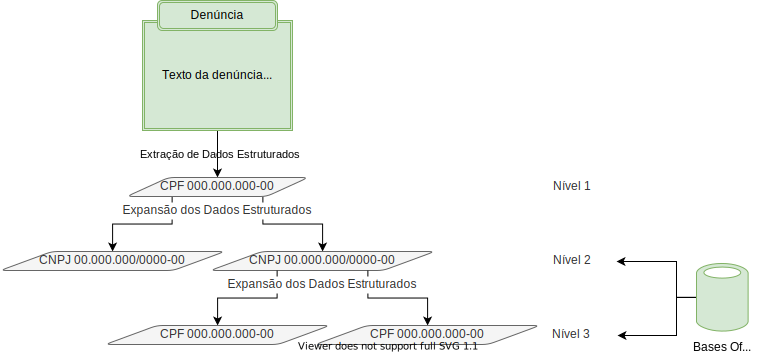
\includegraphics[width=\columnwidth]{images/fig_00200_extracao_expansao.png}
    \end{center}
\legend{Fonte: Autor.}
\end{figure}

A \autoref{fig_00200_extracao_expansao} apresenta um exemplo fictício no qual o processo de extração encontra um CPF. A partir deste CPF dois CNPJs, nos quais o CPF pertence ao quadro societário, são encontrados. Para cada CNPJ encontrado busca-se os CPFs dos demais sócios. Assim, os dados estruturados provenientes da extração são definidos como nível 1, seus dados estruturados derivados nível 2 e assim por diante. Avaliou-se que, acima do nível 3, a quantidade de dados estruturados aumentaria demasiadamente e os mesmos teriam pouca relevância. Assim, na base de dados utilizada para este trabalho serão expandidos e trabalhados apenas informações até o terceiro nível.

\subsection{Qualificação dos Dados Estruturados Encontrados}

O processo de qualificação tem por objetivo extrair outras características para cada dado estruturado encontrado, independentemente do nível. Assim, para um CPF encontrado, por exemplo, pode-se extrair informações como: é ou não servidor público federal, foi demitido da administração pública federal, possui processo administrativo disciplinar, é pessoa exposta politicamente, fez doações a partidos políticos (valor total das doações), entre outras. 

No caso de um CNPJ, como exemplo, podemos verificar se a empresa consta no \sigla{CADIN}{Cadastro Informativo de Créditos não Quitados do Setor Público Federal}, \sigla{CEPIM}{Cadastro de Entidades Privadas sem Fins Lucrativos}, se já teve outras sanções feitas pela administração pública federal, se a empresa fez doações a partidos políticos, entre outras.

As qualificações encontradas podem ser utilizadas como \textit{features} das denúncias.

\subsection{Preparação do \textit{Dataset}}

Esta etapa consiste na consolidação, em \textit{features} ou características, de todas as informações encontradas nas etapas anteriores. Assim, realiza-se um agrupamento por origem de informações. Algumas características como materialidade são somadas outras como CPF de servidor público são contabilizadas. Dessa forma, para cada denúncia, há um registro com uma quantidade grande de colunas nas quais consolidam-se todas as informações encontradas nas etapas anteriores. Por fim, inclui-se o rótulo. A \autoref{tab_00100_visao_geral_dataset} apresenta uma visão em alto nível de como o \textit{dataset} é montado bem como uma explicação da origem de algumas \textit{features} e sua forma de consolidação. 


\begin{table}[htbp]
\caption{Visão geral do dataset após o processamento das denúncias}
\label{tab_00100_visao_geral_dataset}
\tiny
\centering
\begin{tabular}{p{0.175\columnwidth}p{0.55\columnwidth}p{0.2\columnwidth}}
\toprule
     \textit{Feature} &
     Descrição &
     Forma de Consolidação \\
\midrule

    grau\_aptidao &
    Rótulo definido pelos especialistas &
    Único por denúncia \\
      
    txt\_denuncia &
    Conteúdo da denúncia &
    Único por denúncia \\
    
    txt\_anexos & 
    Conteúdo textual extraído dos anexos 
    &  Único por denúncia \\
    
    nome\_em\_denuncia 
    &  Nomes de pessoas encontrados no texto ou anexos da denúncia. São contabilizados apenas nomes existentes na tabela de pessoa física da receita federal
    & Contagem de ocorrências\\
    
    cpf\_em\_texto\_denuncia
    &  CPFs encontrados no texto ou anexos da denúncia
    & Contagem de ocorrências \\
    
    materialidade
    & Referências a valores monetários encontrados diretamente no texto da denúncia e seus anexos ou em contratos e convênios extraídos das mesmas
    & Soma dos valores \\
    
    denuncia\_anonima
    & Indicador se a denúncia é anônima ou não
    & Binário (1 ou 0) \\
    
    ... 
    &  ... 
    & ... \\
    
    palavras\_fortes
    &  Palavras fortes que possam levar ao entendimento de que há ato suspeito sendo denunciado (fraude, ilegal, desvio, superfaturamento, etc.)
    & Contagem de ocorrências \\
    
\bottomrule
\end{tabular}
\legend{Fonte: Autor.}
\end{table}%


Além das 7 \textit{features} e da variável alvo (rótulo) detalhadas na \autoref{tab_00100_visao_geral_dataset}, são extraídas outras 71 \textit{features}. O presente trabalho não detalhará as demais por questões de sigilo, considerando que a metodologia proposta será adotada na instituição em que o autor é vinculado.

Com o dataset finalizado pode-se iniciar a avaliação dos dados para a proposição de um modelo de classificação.

\chapter{Avaliação}
\label{chapter:avaliacao}
\section{Considerações Iniciais}

Neste capítulo, serão descritos os recursos de hardware e software utilizados, o detalhamento da metodologia utilizada, os experimentos realizados, as métricas utilizadas e o modelo escolhido. Por fim, serão exibidos alguns resultados obtidos a partir da utilização do modelo selecionado aplicado em dados reais.

\section{Recursos Utilizados}
\label{section:recursos_utilizados}

Para a realização dos experimentos, utilizou-se um computador com processador Intel(R) Core(TM) i7-7700HQ CPU @ 2.80GHz de 8 núcleos lógicos (4 núcleos físicos com  \textit{hyperthreading}), com 32 GB de memória RAM e 500 GB de SSD. O sistema operacional utilizado foi o Windows 10 Home 64 bits. Utilizou-se a distribuição Anaconda (Python 3.7, 64 bits). As principais bibliotecas Python utilizadas são listadas as seguir:

\begin{itemize}
    \item imbalanced-learn==0.7.0;
    \item joblib==0.17.0;
    \item lightgbm==3.0.0;
    \item numpy==1.19.2;
    \item pandas==1.1.3;
    \item scikit-learn==0.23.2;
    \item scikit-optimize==0.8.1;
    \item scipy==1.5.3;
    \item tika==1.24;
    \item xgboost==1.2.1.
\end{itemize}

\section{Experimentos Propostos}
\label{section:experimentos_propostos}

Nesta seção, serão exploradas algumas possibilidades de uso das informações extraídas para construir classificadores. Desta forma, identificam-se algumas alternativas óbvias que devem ser avaliadas em um primeiro momento.

A primeira trata-se de tentar construir um modelo apenas utilizando os dados estruturados extraídos dos textos. A segunda, tentar construir um modelo apenas com as informações textuais contidas nas denúncias e seus anexos. Por fim, uma combinação de ambas as alternativas.

Como mencionado na \autoref{fig_00100_quantidade_denuncias}, a distribuição de denúncias de acordo com os rótulos não é balanceada. Além disso, algumas classes possuem muito poucas observações. Por essa razão, decidiu-se trabalhar com apenas duas classes apta (1), não apta (0). Rótulos com valor entre 10 e 50 foram considerados como 0 e rótulos com valores entre 60 e 100 foram considerados como 1. A figura \autoref{fig_00300_rotulos_duas_classes} apresenta a distribuição das denúncias considerando apenas duas classes. Apesar de o \textit{dataset} permanecer desbalanceado, a quantidade de denúncias por classe agora é representativa.

\begin{figure}[htbp]
    \caption{Distribuição das denúncias por rótulo utilizando 2 classes}
    \label{fig_00300_rotulos_duas_classes}
    \begin{center}
        \includegraphics[width=300pt]{images/fig_00300_rotulos_duas_classes.png}
    \end{center}
\legend{Fonte: Autor.}
\end{figure}

Neste estudo, não há a necessidade de análise e tratamento de dados faltantes. A razão para isso é que todas as informações são obtidas a partir dos textos e anexos das denúncias. Assim, no caso de textos curtos com poucas informações e nenhum anexo a denúncia tende a ser rejeitada, por que poucos ou nenhum dado estruturado é extraído e o próprio texto não traz elementos suficientes para uma apuração. Assim, a maior parte ou todas as \textit{features} de dados estruturados acabam tendo o seu valor zerado. Além disso o TF-IDF gerado para o modelo textual tende a trazer a maior parte de suas \textit{features} com valores baixos ou zerados.

\subsection{Definições Metodológicas}
\label{section:definicoes_metodologicas}

Conforme já informado no \autoref{chapter:metodologia_proposta}, o \textit{dataset} utilizado possui 1489 registros de denúncias rotuladas como apuráveis (aptas) ou não apuráveis (não aptas). Assim, separou-se 80\% (1191) dos registros em um \textit{dataset} de treinamento e 20\% dos registros (298) em um \textit{dataset} de testes. Além disso, a separação em conjuntos de treinamento e testes foi estratificada, isto é, manteve-se a mesma proporção de registros do \textit{dataset} original, para as classes positiva (apurável) e negativa (não apurável), em ambos os conjuntos.

Todos os procedimentos relacionados a seleção de \textit{features}, seleção de modelos e \textit{tunning} de hiper-parâmetros foram realizados utilizando-se o \textit{dataset} de treinamento e as avaliações de desempenho foram realizadas utilizando-se validação cruzada no próprio \textit{dataset} de treinamento. O \textit{dataset} de testes foi utilizado apenas para aferir os scores finais dos modelos.

\subsection{Modelo considerando apenas os dados estruturados}
\label{section:modelo_dados_estruturados}

A primeira tarefa realizada nesta etapa foi a avaliação da representatividade das \textit{features} obtidas na tentativa de explicar a variável alvo. O objetivo é diminuir a complexidade do modelo. Por questões de objetividade e tempo, optou-se por um processo automatizado.

O processo escolhido utiliza a classe \textit{SelectFromModel} da biblioteca \textit{scikit-learn} do Python \cite{scikit-learn}. Esta classe foi utilizada para selecionar as '\textit{k}' melhores \textit{features} após o treinamento de um \textit{RandomForestClassifier} \cite{breiman2001random}. Estas informações ficam armazenadas no atributo \textit{feature\_importances\_} do modelo. Foram realizados 39 testes para $for\ _k = 2,...,78\ \forall\ k=2n,\ n \in \mathbb{N}$.

Em cada iteração, é criada uma instância da classe \textit{SelectFromModel} com o parâmetro $max\_features = k$, equivalente a iteração. A classe então é utilizada para selecionar as k melhores \textit{features} e transformar o \textit{dataset} de treino para descartar aquelas não selecionadas. Com o \textit{dataset} de treino transformado, treina-se um novo \textit{RandomForestClassifier} e realiza-se a avaliação do modelo de acordo com as métricas de \textit{Average Precision}, \textit{Balanced Accuracy} e \textit{ROC AUC}. A tabela \autoref{tab_00200_metricas_numero_features} e a \autoref{fig_00040_kneeplot} apresentam um resumo dos resultados obtidos.

\begin{table}[htbp]
\caption{Métricas de acordo com o número de \textit{features}}
\label{tab_00200_metricas_numero_features}
\small
\centering
\begin{tabular}{rrrr}
\toprule
 Número de \textit{Features} &  Average Precision &  Balanced Accuracy &  ROC AUC  \\
\midrule
                 
                 10 &           0.538429 &           0.623408 &  0.721747 \\
                 \textbf{20} &           
                 \textbf{0.581019} &           
                 \textbf{0.647302} &  
                 \textbf{0.741056} \\
                 30 &           0.579207 &           0.651423 &  0.740430 \\
                 40 &           0.578372 &           0.657877 &  0.739688 \\
                 50 &           0.584122 &           0.654597 &  0.739786 \\
                 60 &           0.584938 &           0.653307 &  0.739417 \\
                 70 &           0.587008 &           0.654857 &  0.740949 \\
\bottomrule
\end{tabular}
\legend{Fonte: Autor.}
\end{table}%

\begin{figure}[htbp]
    \caption{Métricas de acordo com o número de \textit{features}}
    \label{fig_00040_kneeplot}
    \begin{center}
        \includegraphics[width=\columnwidth]{images/fig_00040_kneeplot.png}
    \end{center}
\legend{Fonte: Autor.}
\end{figure}

Com base nos resultados avaliou-se que, a partir de 20 \textit{features}, o ganho dos scores não é tão relevante e a utilização do conjunto completo aumentaria o tempo de treinamento e a complexidade do modelo. Assim, escolheu-se utilizar as 20 mais relevantes na etapa de modelagem.

A decisão sobre qual algoritmo utilizar para a geração do modelo foi tomada com base na comparação do score de área sob a curva ROC (\textit{roc\_auc}) obtido em diversos modelos testados. Esta métrica foi escolhida por ser uma métrica interessante para avaliação do desempenho do modelo com foco na classe positiva, neste caso a classe 1.

O processo consistiu basicamente em realizar as seguintes etapas para cada algoritmo a ser avaliado:

\begin{itemize}
    \item utilizar a classe \textit{GridSearchCV}, do \textit{scikit-learn} com algumas combinações de hiper-parâmetros e validação cruzada com 10 partições estratificadas para escolher um boa versão de modelo e tornar mais justa a comparação;
    
    \item utilizar a melhor combinação de hiper-parâmetros encontrada para realizar uma validação cruzada com 10 partições e obter as seguintes métricas: \textit{roc\_auc}, \textit{balanced\_accuracy}, \textit{average\_precision} e \textit{f1\_weighted};
    
    \item utilizar a distribuição de scores obtidos para cada métrica e modelo para realizar a escolha do algoritmo mais adequado ao problema.
\end{itemize}

A \autoref{fig_00400_comparacao_score_modelos_dados_estr} apresenta um gráfico de \textit{boxplot} para cada algoritmo avaliado. A ordem em que os algoritmos aparecem, em todos os gráficos, foi definida através do score obtido pela métrica \textit{roc\_auc}, em ordem decrescente, da esquerda para a direita. \newline


\begin{figure}[htbp]
    \caption{Distribuição dos scores por métrica e modelo}
    \label{fig_00400_comparacao_score_modelos_dados_estr}
    \begin{center}
        \includegraphics[width=\columnwidth]{images/fig_00400_comparacao_score_modelos_dados_estr.png}
    \end{center}
\legend{Fonte: Autor.}
\end{figure}

O algoritmo escolhido foi o \textit{RandomForestClassifier}, por apresentar o melhor desempenho pela métrica escolhida. Além disso, o algoritmo também teve uma boa performance nas outras três métricas avaliadas. 

O passo seguinte foi a otimização dos hiper-parâmetros. Utilizou-se a biblioteca \textit{skopt} para realizar uma busca automática. Por fim, um novo modelo foi treinado utilizando-se os parâmetros selecionados e todos os dados de treinamento. A \autoref{tab_00300_desempenho_final_modelo_dados_estr} apresenta a matriz de confusão e a \autoref{tab_00400_desempenho_final_modelo_dados_estr} apresenta o relatório de classificação, provenientes das previsões do modelo para os dados de teste.

\begin{table}[htbp]
\caption{Matriz de confusão do modelo, avaliando-se pelos dados de teste}
\label{tab_00300_desempenho_final_modelo_dados_estr}
\small
\centering
\begin{tabular}{lrr}
\toprule
      {} &  Predito como 0 &  Predito como 1 \\
\midrule
Classe 0 &             188 &              32 \\
Classe 1 &              28 &              50 \\
\bottomrule
\end{tabular}
\legend{Fonte: Autor.}
\end{table}%

\begin{table}[htbp]
\caption{Relatório de classificação, avaliando-se pelos dados de teste}
\label{tab_00400_desempenho_final_modelo_dados_estr}
\small
\centering
\begin{tabular}{lrrrr}
\toprule
          {} & Precisão   &  Revocação & F1-Score &  Suporte \\
\midrule
       Classe 0 &      0,87  &    0,85    &     0,86 &      220 \\
       Classe 1 &      0,61  &    0,64    &     0,62 &       78 \\
             {} &        {}  &      {}    &       {} &       {} \\
       Acurácia &        {}  &      {}    &     0,80 &      298 \\
          Média &      0,74  &    0,75    &     0,74 &      298 \\
Média Ponderada &      0,80  &    0,80    &     0,80 &      298 \\
\bottomrule
\end{tabular}
\legend{Fonte: Autor.}
\end{table}%

O conjunto de testes utilizado possui 298 registros. Assim, como é possível observar na \autoref{tab_00300_desempenho_final_modelo_dados_estr}, tem-se 188 verdadeiros negativos e 50 verdadeiros positivos que somam um total de 238 classificações corretas. Ao avaliar os resultados por classe (\autoref{tab_00400_desempenho_final_modelo_dados_estr}), observa-se que o modelo possui uma precisão para a classe 0 (0,87) bem superior à da classe 1 (0,61). O modelo apresenta uma acurácia de 0,80, porém, a acurácia balanceada foi de 0,75. O score \textit{roc\_auc} foi de 0.82 e a curva ROC é apresentada na \autoref{fig_00410_roc_auc_dados_estr}.

\begin{figure}[htbp]
    \caption{Curva Característica de Operação do Receptor (ROC)}
    \label{fig_00410_roc_auc_dados_estr}
    \begin{center}
        \includegraphics[width=\columnwidth]{images/fig_00410_roc_auc_dados_estr.png}
    \end{center}
\legend{Fonte: Autor.}
\end{figure}

Pela análise da curva ROC, entende-se que seria possível elevar o \textit{recall} do modelo diminuindo-se o limiar utilizado para computar as classes positivas e negativas. Com o limiar em 0,5 (padrão), tem-se uma taxa de falsos positivos de 0,14 e um \textit{recall} de 0,64. Entretanto, ao mover-se o limiar para 0.37, tem-se uma taxa de falsos positivos de 0,28 e um \textit{recall} de 0,76. Talvez seja um \textit{tradeoff} interessante pois o falso positivo de uma denúncia é menos problemático do que um falso negativo.

Em geral, avalia-se que a capacidade de distinção entre as classes, aprendida pelo modelo, é bastante razoável.

\subsection{Modelo considerando apenas os textos}
\label{section:modelo_texto}

Nesta seção será avaliada a possibilidade de criação de um modelo utilizando apenas os textos das denúncias e de seu anexos. Como foi visto no \autoref{chapter:revisao_bibliografica}, há diferentes formas de extrair informações de textos. Elas variam bastante de acordo com o propósito pretendido. 

Primeiramente realizou-se um pré-processamento em todos os documentos com o objetivo de padronizar os textos. Todas as letras foram convertidas para minúsculas, caracteres acentuados foram substituídos por seus equivalentes sem acentuação, \textit{stopwords} foram removidas e espaços excessivos foram eliminados.

Para o propósito deste estudo, será avaliado o TF-IDF como técnica para extração de características de documentos. Como explicado anteriormente, esta técnica combina a contagem de palavras presentes no texto com a ocorrência das mesmas em outros documentos. Com isso, palavras que ocorrem em muitos documentos terão seu peso atenuado enquanto que palavras que ocorrem um conjuntos pequenos de documentos receberão um peso maior.
Como exemplo, a \autoref{tab_00500_exemplo_tfidf} exibe algumas \textit{features} geradas pelo TF-IDF para as primeiras 10 denúncias do \textit{dataset} de treinamento.

\begin{table}[htbp]
\caption{Exemplo de \textit{features} geradas pelo TF-IDF}
\label{tab_00500_exemplo_tfidf}
\tiny
\centering
\begin{tabular}{lrrrrrrrrrrl}
\toprule
 ... &  ativo &    ato &   atos &  atraves &  atribuicoes &  atuacao &  atual &  auditoria &  augusto &  ausencia &  ... \\
\midrule
... & 0,0000 & 0,0988 & 0,0658 &   0,0036 &       0,0115 &   0,0069 & 0,0156 &     0,0000 &   0,0000 &    0,0266 &  ... \\
 ... & 0,0084 & 0,0449 & 0,0184 &   0,0090 &       0,0107 &   0,0045 & 0,0000 &     0,0000 &   0,0027 &    0,0000 &  ... \\
 ... & 0,0000 & 0,0000 & 0,0000 &   0,0000 &       0,0000 &   0,0000 & 0,0000 &     0,0000 &   0,0000 &    0,0000 &  ... \\
 ... & 0,0000 & 0,0000 & 0,0000 &   0,1386 &       0,0000 &   0,0000 & 0,0000 &     0,0000 &   0,0000 &    0,0000 &  ... \\
 ... & 0,0000 & 0,0320 & 0,0145 &   0,0158 &       0,0029 &   0,0087 & 0,0074 &     0,0000 &   0,0007 &    0,0000 &  ... \\
 ... & 0,0000 & 0,0000 & 0,0000 &   0,0000 &       0,0000 &   0,0000 & 0,0000 &     0,0000 &   0,0000 &    0,0000 &  ... \\
 ... & 0,0000 & 0,0000 & 0,0000 &   0,0000 &       0,0000 &   0,0000 & 0,0000 &     0,0000 &   0,0000 &    0,0000 &  ... \\
 ... & 0,0000 & 0,0001 & 0,0002 &   0,0001 &       0,0000 &   0,0003 & 0,0000 &     0,0000 &   0,0006 &    0,0000 &  ... \\
 ... & 0,0000 & 0,0000 & 0,0000 &   0,0000 &       0,0000 &   0,0000 & 0,1226 &     0,0000 &   0,0000 &    0,0000 &  ... \\
 ... & 0,0000 & 0,0000 & 0,0000 &   0,0000 &       0,0000 &   0,0000 & 0,0000 &     0,0000 &   0,0000 &    0,0000 &  ... \\
\bottomrule
\end{tabular}
\legend{Fonte: Autor.}
\end{table}%

Na \autoref{tab_00500_exemplo_tfidf}, cada linha representa uma denúncia e cada coluna representa uma palavra. Palavras que não são encontradas na denúncia recebem um peso 0 e palavras que estão presentes na denúncia recebem um peso que é ponderado pela quantidade de vezes que ela está presente no texto e, também, pela sua presença ou não nas demais denúncias analisadas. Esta matriz de palavras por documento será utilizada para o treinamento e comparação dos modelos. Para a comparação dos algoritmos, o TF-IDF foi parametrizado de forma a permitir no máximo 5.000 palavras e só serão aceitas palavras que ocorram, em pelo menos 5 documentos ou no máximo em 50\% dos documentos. Assim, elimina-se palavras que não discriminam muito bem grupos de documentos por serem específicas demais ou genéricas demais.

A mesma metodologia utilizada na escolha do algoritmo na \autoref{section:modelo_dados_estruturados} foi utilizada para a escolha do algoritmo para este modelo.  A \autoref{fig_00500_comparacao_score_modelos_texto} apresenta um gráfico de \textit{boxplot} com o desempenho de cada modelo. Os modelos foram ordenados na figura pela métrica \textit{roc\_auc}, em ordem decrescente, da esquerda para a direita. O algoritmo que teve o melhor desempenho foi o \textit{XGBClassifier} com um \textit{score} de 0,830. Além disso, teve ainda, o melhor desempenho nas outras métricas avaliadas. Por essa razão, escolheu-se o \textit{XGBClassifier} para a otimização de hiper-parâmetros e avaliação final.

\begin{figure}[htbp]
    \caption{Distribuição dos scores por métrica e modelo }
    \label{fig_00500_comparacao_score_modelos_texto}
    \begin{center}
        \includegraphics[width=\columnwidth]{images/fig_00500_comparacao_score_modelos_texto.png}
    \end{center}
\legend{Fonte: Autor.}
\end{figure}

O mesmo processo de otimização utilizado para o modelo da \autoref{section:modelo_dados_estruturados} foi adotado para este modelo. Assim, após a execução da biblioteca \textit{skopt} para encontrar bons hiper-parâmetros para o modelo, foi gerado um modelo treinado com todos os dados de treinamento. Os resultados são exibidos nas tabelas \ref{tab_00600_desempenho_final_modelo_texto} e \ref{tab_00700_desempenho_final_modelo_texto}.


\begin{table}[htbp]
\caption{Matriz de confusão do modelo, avaliando-se pelos dados de teste}
\label{tab_00600_desempenho_final_modelo_texto}
\small
\centering
\begin{tabular}{lrr}
\toprule
      {} &  Predito como 0 &  Predito como 1 \\
\midrule
Classe 0 &             187 &              33 \\
Classe 1 &              31 &              47 \\
\bottomrule
\end{tabular}
\legend{Fonte: Autor.}
\end{table}%

\begin{table}[htbp]
\caption{Relatório de classificação, avaliando-se pelos dados de teste}
\label{tab_00700_desempenho_final_modelo_texto}
\small
\centering
\begin{tabular}{lrrrr}
\toprule
             {} & Precisão   &  Revocação & F1-Score &  Suporte \\
\midrule
       Classe 0 &      0,86  &    0,85    &     0,85 &     220 \\
       Classe 1 &      0,59  &    0,60    &     0,59 &       78 \\
             {} &        {}  &      {}    &       {} &       {} \\
       Acurácia &        {}  &      {}    &     0,79 &      298 \\
          Média &      0,72  &    0,73    &     0,72 &      298 \\
Média Ponderada &      0,79  &    0,79    &     0,79 &      298 \\
\bottomrule
\end{tabular}
\legend{Fonte: Autor.}
\end{table}%


É possível observar na matriz de confusão (\autoref{tab_00600_desempenho_final_modelo_texto}) 187 verdadeiros negativos e 47 verdadeiros positivos que somam um total de 234 classificações corretas. Ao avaliar os resultados por classe (\autoref{tab_00700_desempenho_final_modelo_texto}), observa-se que o modelo possui uma precisão para a classe 0 (0,86) bem superior à da classe 1 (0,59). O modelo apresenta uma acurácia de 0,79, porém, a acurácia balanceada foi de 0,73. O score \textit{roc\_auc} foi de 0,83 e a curva ROC é apresentada na \autoref{fig_00600_roc_auc_texto}.

\begin{figure}[htbp]
    \caption{Curva Característica de Operação do Receptor (ROC)}
    \label{fig_00600_roc_auc_texto}
    \begin{center}
        \includegraphics[width=\columnwidth]{images/fig_00600_roc_auc_texto.png}
    \end{center}
\legend{Fonte: Autor.}
\end{figure}

De forma geral, pode-se afirmar que este modelo teve um desempenho bem parecido com o modelo proposto na \autoref{section:modelo_dados_estruturados}. Talvez levemente inferior. Mas, ainda assim, com um poder de discriminação entre as classes razoável, conforme observa-se na \autoref{fig_00600_roc_auc_texto}.

\section{Combinação dos Modelos}
\label{section:combinacao_modelos}

Nesta seção, avalia-se a possibilidade de combinar os modelos obtidos nas seções \ref{section:modelo_dados_estruturados} e \ref{section:modelo_texto}. O objetivo aqui é identificar se algum tipo de combinação pode melhorar o desempenho da classificação em relação aos desempenhos isolados de cada modelo. 

Após aplicar-se as correlações de Pearson e Spearman nas probabilidades (para a classe positiva) previstas pelos dois modelos, para os dados de teste, obtém-se, respectivamente, os coeficientes 0,6879 e 0,6419. Por esta razão, entende-se que há uma certa quantidade de registros nos quais os modelos possivelmente classificam de forma diferente. Assim, foram testadas 3 combinações possíveis. A menor, a maior e a média das probabilidades, para a classe positiva, previstas pelos dois modelos, para cada registro do conjunto de testes.


\subsection{Combinação dos modelos pela menor probabilidade}

Neste cenário, foram aplicados os dois modelos nos dados de teste. Para cada registro utilizou-se a menor probabilidade obtida entre os modelos e a outra foi descartada. Entende-se que, neste caso, tem-se uma classificação mais pessimista ou conservadora pois se, ao menos, um dos modelos indicar uma probabilidade abaixo de 0,5, o registro será classificado como pertencente à classe 0. O resultado desta combinação pode ser avaliado nas tabelas \ref{tab_00800_desempenho_final_modelo_comb_menor} e \ref{tab_00900_desempenho_final_modelo_comb_menor}.

\begin{table}[htbp]
\caption{Matriz de confusão do modelo, avaliando-se pelos dados de teste}
\label{tab_00800_desempenho_final_modelo_comb_menor}
\small
\centering
\begin{tabular}{lrr}
\toprule
      {} &  Predito como 0 &  Predito como 1 \\
\midrule
Classe 0 &             204 &              16 \\
Classe 1 &              39 &              39 \\
\bottomrule
\end{tabular}
\legend{Fonte: Autor.}
\end{table}%

\begin{table}[htbp]
\caption{Relatório de classificação, avaliando-se pelos dados de teste}
\label{tab_00900_desempenho_final_modelo_comb_menor}
\small
\centering
\begin{tabular}{lrrrr}
\toprule
             {} & Precisão   &  Revocação & F1-Score &  Suporte \\
\midrule
       Classe 0 &      0,84  &    0,93    &     0,88 &      220 \\
       Classe 1 &      0,71  &    0,50    &     0,59 &       78 \\
             {} &        {}  &      {}    &       {} &       {} \\
       Acurácia &        {}  &      {}    &     0,79 &      298 \\
          Média &      0,77  &    0,71    &     0,73 &      298 \\
Média Ponderada &      0,81  &    0,82    &     0,80 &      298 \\
\bottomrule
\end{tabular}
\legend{Fonte: Autor.}
\end{table}%

Esta combinação leva o modelo, de uma forma geral, a rejeitar mais denúncias. Isso ocasiona um aumento de precisão para ambas as classes, entretanto, a revocação ou taxa de verdadeiros positivos cai bastante. Neste caso tem-se um aumento considerável na quantidade de falsos negativos. Esse comportamento não é interessante para o problema em questão. O \textit{ROC AUC score} foi de 0,83 o \textit{balanced accuracy score} foi de 0,71. Houve uma melhora na métrica ROC AUC e uma piora na acurácia balanceada quando comparado com os modelos das seções \ref{section:modelo_dados_estruturados} e \ref{section:modelo_texto}.

\subsection{Combinação dos modelos pela maior probabilidade}

Neste cenário, utilizou-se, para cada registro a maior probabilidade obtida entre os modelos e a outra foi descartada. Entende-se que, neste caso, tem-se uma classificação mais otimista ou arrojada pois se, ao menos, um dos modelos indicar uma probabilidade acima de 0,5, o registro será classificado como pertencente à classe 1. O resultado desta combinação pode ser avaliado nas tabelas \ref{tab_001000_desempenho_final_modelo_comb_maior} e \ref{tab_001100_desempenho_final_modelo_comb_maior}.

\begin{table}[htbp]
\caption{Matriz de confusão do modelo, avaliando-se pelos dados de teste}
\label{tab_001000_desempenho_final_modelo_comb_maior}
\small
\centering
\begin{tabular}{lrr}
\toprule
      {} &  Predito como 0 &  Predito como 1 \\
\midrule
Classe 0 &             171 &              49 \\
Classe 1 &              20 &              58 \\
\bottomrule
\end{tabular}
\legend{Fonte: Autor.}
\end{table}%

\begin{table}[htbp]
\caption{Relatório de classificação, avaliando-se pelos dados de teste}
\label{tab_001100_desempenho_final_modelo_comb_maior}
\small
\centering
\begin{tabular}{lrrrr}
\toprule
             {} & Precisão   &  Revocação & F1-Score &  Suporte \\
\midrule
       Classe 0 &      0,90  &    0,78    &     0,83 &      220 \\
       Classe 1 &      0,54  &    0,74    &     0,63 &       78 \\
             {} &        {}  &      {}    &       {} &       {} \\
       Acurácia &        {}  &      {}    &     0,77 &      298 \\
          Média &      0,72  &    0,76    &     0,73 &      298 \\
Média Ponderada &      0,80  &    0,77    &     0,78 &      298 \\
\bottomrule
\end{tabular}
\legend{Fonte: Autor.}
\end{table}%

Esta combinação leva o modelo, de uma forma geral, a aceitar mais denúncias. Isso ocasiona uma diminuição de precisão para a classe positiva, entretanto, a revocação ou taxa de verdadeiros positivos aumenta consideravelmente. Neste caso, tem-se um aumento considerável na quantidade de falsos positivos. Esse comportamento pode ser aceitável para o problema em questão. O \textit{ROC AUC score} foi de 0,85 o \textit{balanced accuracy score} foi de 0,76. Houve uma melhora em ambas as métricas quando comparado com os modelos das seções \ref{section:modelo_dados_estruturados} e \ref{section:modelo_texto}.


\subsection{Combinação dos modelos pela média das probabilidades}

Neste cenário, utilizou-se, para cada registro a média das probabilidades obtidas entre os modelos. Entende-se que, neste caso, tem-se uma classificação mais equilibrada. O resultado desta combinação pode ser avaliado nas tabelas \ref{tab_001200_desempenho_final_modelo_comb_media} e \ref{tab_001300_desempenho_final_modelo_comb_media}.

\begin{table}[htbp]
\caption{Matriz de confusão do modelo, avaliando-se pelos dados de teste}
\label{tab_001200_desempenho_final_modelo_comb_media}
\small
\centering
\begin{tabular}{lrr}
\toprule
      {} &  Predito como 0 &  Predito como 1 \\
\midrule
Classe 0 &             192 &              28 \\
Classe 1 &              34 &              44 \\
\bottomrule
\end{tabular}
\legend{Fonte: Autor.}
\end{table}%

\begin{table}[htbp]
\caption{Relatório de classificação, avaliando-se pelos dados de teste}
\label{tab_001300_desempenho_final_modelo_comb_media}
\small
\centering
\begin{tabular}{lrrrr}
\toprule
             {} & Precisão   &  Revocação & F1-Score &  Suporte \\
\midrule
       Classe 0 &      0,85  &    0,87    &     0,86 &      220 \\
       Classe 1 &      0,61  &    0,56    &     0,59 &       78 \\
             {} &        {}  &      {}    &       {} &       {} \\
       Acurácia &        {}  &      {}    &     0,79 &      298 \\
          Média &      0,73  &    0,72    &     0,72 &      298 \\
Média Ponderada &      0,79  &    0,79    &     0,79 &      298 \\
\bottomrule
\end{tabular}
\legend{Fonte: Autor.}
\end{table}%

Observa-se um equilíbrio maior entre precisão e revocação para ambas as classes. Entretanto há uma diminuição no número de acertos da classe positiva e, consequentemente, um aumento no número de falsos negativos. O \textit{ROC AUC score} foi de 0,86 o \textit{balanced accuracy score} foi de 0,72. Houve uma melhora para ROC AUC e uma piora para a acurácia balanceada quando comparado com os modelos das seções \ref{section:modelo_dados_estruturados} e \ref{section:modelo_texto}.

\section{Discussão}

A escolha de qual modelo seria mais interessante para o problema tem como baliza um ponto muito importante: enviar uma denúncia fraca ou sem elementos para a apuração é um problema muito menor do que não apurar uma denúncia com elementos suficientes e verdadeira.

A \autoref{tab_001400_desempenho_final_tabela_comparativa} apresenta as principais métricas obtidas para cada experimento apresentado nas seções  \ref{section:experimentos_propostos} e \ref{section:combinacao_modelos}.

\begin{table}[htbp]
\caption{Tabela comparativa dos resultados obtidos para cada modelo}
\label{tab_001400_desempenho_final_tabela_comparativa}
\tiny
\centering
\begin{tabular}{lrrrr}
\toprule
            Modelo &  
            Precisão média  &  
            Acurácia Balanceada & 
            F1-Score (Classe Positiva) &  
            ROC AUC \\
\midrule
              Dados Estruturados           &   0,48  &  0,75 & 0,62 & 0,82 \\
                           Texto           &   0,46  &  0,74 & 0,59 & 0,84 \\
  Combinação pela menor probabilidade      &   0,49  &  0,71 & 0,59 & 0,84 \\
  Combinação pela maior probabilidade      &   0,47  &  0,76 & 0,61 & 0,85 \\ 
  Combinação pela média das probabilidades &   0,46  &  0,72 & 0,59 & 0,86 \\ 

\bottomrule
\end{tabular}
\legend{Fonte: Autor.}
\end{table}%


Entende-se que a metodologia proposta atinge o objetivo de melhorar a classificação de denúncias aptas. O modelo baseado apenas nos dados estruturados evidencia esta afirmação. Ou seja, a derivação de informações a partir de elementos chave encontrados nas denúncias efetivamente colabora com o processo de classificação. Ainda assim, ao avaliar-se as previsões obtidas pelos dois modelos, constata-se que, em muitos casos, ambos se complementam. A consequência disso foi um melhor desempenho obtido na combinação otimista destes modelos em relação aos seus desempenhos isolados.

\chapter{Conclusão}
\label{chapter:conclusao}


- a premissa de utilizar o conteúdo da denúncia para classificar a aptidão é válida?
- os modelos se complementam?
- o modelo é util?

- como pode ser melhorado?


- pq combinar?

- dados presentes na denuncia vs dados derivados do que se ve na denuncia 

- modelos se complementam?

% \chapter{Instalando o abnTeX2}
% \label{chapter:instalando-abntex}
% \input{tex/instalando-abntex}

% \chapter{Orientações gerais}
% \label{chapter:orientacoes-gerais}
% \input{tex/orientacoes-gerais}

% \chapter{Configuração dos elementos pré-textuais}
% \label{chapter:config-pre-textual}
% \input{tex/config-pre-textual}

% \chapter{Corpos flutuantes}
% \label{chapter:corpos-flutuantes}
% \input{tex/corpos-flutuantes}

% \chapter{Listas}
% \label{chapter:listas}
% \input{tex/listas}

% \chapter{Ferramentas úteis}
% \label{chapter:ferramentas-uteis}
% \input{tex/ferramentas-uteis}

% \chapter{Citações e referências}
% \label{chapter:citacoes}
% \input{tex/citacoes}


% ---
% Finaliza a parte no bookmark do PDF, para que se inicie o bookmark na raiz
% ---
\bookmarksetup{startatroot}% 
% ---

% ----------------------------------------------------------
% ELEMENTOS PÓS-TEXTUAIS
% ----------------------------------------------------------
\postextual

% ----------------------------------------------------------
% Referências bibliográficas
% ----------------------------------------------------------
\bibliography{99_bibliografia}

% ---------------------------------------------------------------------
% GLOSSÁRIO
% ---------------------------------------------------------------------

% Arquivo que contém as definições que vão aparecer no glossário

\newword{Teste}{teste ...}

\newword{Teste}{teste ...}

\newword{Outlier}{Em estatística, outlier, valor aberrante ou valor atípico, é uma observação que apresenta um grande afastamento das demais da série, ou que é inconsistente}
% Comando para incluir todas as definições do arquivo glossario.tex
\glsaddall
% Impressão do glossário
\printglossaries

% ----------------------------------------------------------
% Apêndices
% ----------------------------------------------------------

% ---
% Inicia os apêndices
% ---
\begin{apendicesenv}

    % \chapter{Documento básico usando a classe \textit{icmc}}
    % \label{chapter:documento-basico}
    % \input{tex/appendix/documento-basico}
    
    % \chapter{Configuração do programa JabRef}
    % \label{chapter:configuracao-jabref}
    % \input{tex/appendix/configuracao-jabref}

\end{apendicesenv}
% ---


% ----------------------------------------------------------
% Anexos
% ----------------------------------------------------------

% ---
% Inicia os anexos
% ---
\begin{anexosenv}

    \chapter{Páginas interessantes na Internet} 
    \label{chapter:paginas-interessantes}
    \input{tex/annex/paginas-interessantes}

\end{anexosenv}
% ---

\end{document}